\chapter{Testing}

\section{MPU}
In order to test the memory partition mapping, for an amount of space given, it's used a non-specific initial
 pointer representing the begining of the memory free space, specific sizes for each partition and it's
  writen in each memory position the number of the partition that is ocupied with. At the end, the
   whole memory avaiable for the test is printed and confirmed if the space given for each is enough and if they are allocated in the right place.\\
  If the amount of memory needed is bigger than the memory given a segmentation fault occurs.\\
 The tests cover the different partition memory distribuitions and sizes in memory, for the 3 cases of not
  having 1, 2 or  3 subregions used by the main partition of the region. For that we used 5 partitions, with
   specific memory requirements, in order to test the different memory alloctions combinations.\\
  The results printed showed us that the new sizes and subregions distribution allowing to have the less
  spare memory possible, comparing with the theoretical calculations.\\
\begin{figure}[H]
\centering
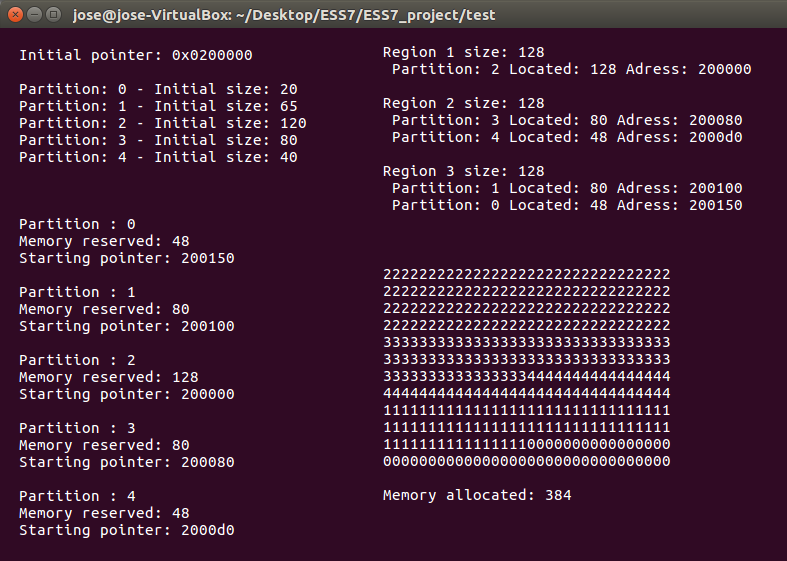
\includegraphics[width=15cm]{mpu_test.png}
\captionof{figure}{Terminal displaying the results}
\label{fig:testing_mpu}
\end{figure}


\section{XML validation}
Currently there is no validation of the XML file.
The XML is currently prone to human error when manually
adding to the file, also it does not prevent elements
not compliant with the schema being written.


\section{Scheduler}
The scheduler has been tested to work provided the XML file specifies reasonable
windows. The scheduler has not been tested with edge cases.\\
The kernel does not record any runtime metrics. Empirical
evidence shows that the scheduler is working according to the windows specified in the
XML schema and according to the designed algorithms. Window durations is
scaled up to make it possible with the human eye to determine that the scheduler
indeed follows the windows.


\section{\arinc{} specification - Part 3}
In order to test a system for compliance with \arinc{},
the authors of the standard provide a conformity test
specification. This is a separate document, as a part of the
\arinc{} specification:
\begin{itemize}
	\item\textbf{Part 0} Introduction to ARINC 653
	\item\textbf{Part 1} Required services. This includes system services,
	data structures and functional behaviour.
	\item\textbf{Part 2} Extended services. For example file handling or external events
	\item\textbf{Part 3} \textbf{Conformity test}
	\item\textbf{Part 4} Subset Services
	\item\textbf{Part 5} Core Software Recommended Capabilities
\end{itemize}

Software developers should use this to test the compliance with
Part 1 of the standard. This could be done in the future phases of the \OSname{} OS in order
to demonstrate full compliance of the APEX behavior.


\section{Interpartition Communication}
Interpartition Communication is tested for queuing ports, not sampling ports.
The test is done with the three partitions \texttt{red\_toggler},
\texttt{yellow\_toggler} and \texttt{stdio\_sys}. \texttt{red\_toggler} and
\texttt{yellow\_toggler} broadcast their respective partition name as a string
to the \texttt{stio\_channel}. The \texttt{stdio\_sys} reads any message within its
time-frame and transmits the strings by UART to a connected terminal. Both
transmitting partitions are set to transmit their string every two seconds. A
sample of a recorded output is depicted in figure \ref{fig:message_test},
showing that the communication scheme works as intended.

\begin{figure}[H]
	\centering
	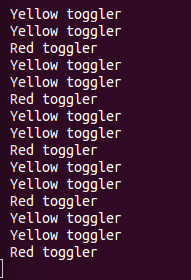
\includegraphics[scale=0.5]{message_test.png}
	\caption{Terminal showing the strings originating from two different
		partitions.}
	\label{fig:message_test}
\end{figure}

As can be seen from the figure, the \texttt{yellow\_toggler} is sending twice as
many messages as \texttt{red\_toggler}. This is due to the scheduling of the two
partitions. The file main\_schema.xml shows that both partitions are
scheduled to execute twice within the major time-frame of 20 seconds, but that
\texttt{yellow\_toggler} is given twice the time of \texttt{red\_toggler} at
every interval and hence gets to print more often.\\

Even though the sampling port module is implemented in the codebase, it is yet
to be fully integrated into \OSname{} and therefore is not tested.
